\documentclass[12pt]{article}
\usepackage{graphicx}
\usepackage[dvips]{psfrag}
\begin{document}
\raggedright
\psfrag{a}{$a$}
\psfrag{b}{$b$}
\psfrag{B}{$\beta$}
\psfrag{f(a)}{$f(a)$}
\psfrag{f(b)}{$f(b)$}
\psfrag{f(u)}{$f(u)$}
\psfrag{f(x)}{$f(x)$}
\psfrag{u}{$u$}
\psfrag{x}{$x$}
\psfrag{y}{$\gamma$}
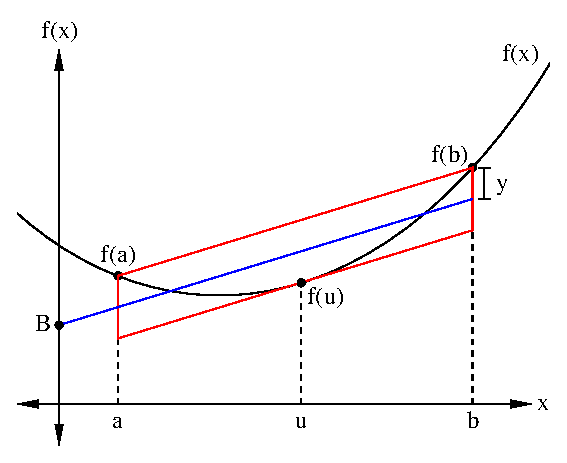
\includegraphics{diagram.eps}

For $\hat{x} = [a..b]$, if $0 \notin f''(\hat{x})$, then the affine approximation $f_a(\hat{x}) = \alpha \hat{x} + \beta + \gamma \varepsilon_k$, where
$\varepsilon_k$ is a new noise variable. $r(x)$ is the line interpolating the
points $(a, f(a))$ and $(b, f(b))$.
\begin{eqnarray*}
f'(u) & = & \alpha \\
\alpha & = & {{f(b) - f(a)} \over {b - a}} \\
\beta & = & {{f(u) + r(u)} \over 2} - \alpha u \\
\gamma & = & {{|f(u) - r(u)|} \over 2} \\
\end{eqnarray*}

\newpage
Canonical function:
\begin{verbatim}
Affine& fooA (Affine& a)
{
  if (interval outside of domain)
    throw Affine::DomainError();
  if (a.lo() == a.hi())
    a = std::foo(a.lo());
  else {
    Interval range(foo(Interval(a)));
    Real f_lo = std::foo(a.lo()),
    f_hi = std::foo(a.hi()),
    slope = (f_hi - f_lo) / (a.hi() - a.lo()),
    u = f_deriv_inv(slope), // inverse of derivative of foo
    f_0 = std::foo(u) - slope * u,
    r_0 = f_lo - slope * a.lo(),
    intercept = 0.5 * (f_0 + r_0),
    error = 0.5 * (f_0 - r_0);

    a.calc(&slope, &intercept, &error, &range);
  }
  return a;
}
\end{verbatim}

\end{document}
